\subsection{Kuroda Transformation}

Die   Umwandlung   von   LC-Filter   in   Leitungsfilter    ist    dank    der
Richards-Transformation recht einfach, jedoch  wird  man  bei der Realisierung
als Mikrostreifenfilter auf Probleme stossen.

\begin{figure}[h!]
    \centering
    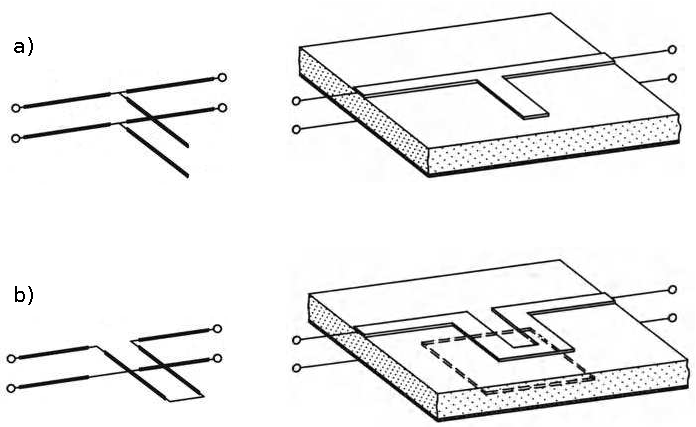
\includegraphics[width=\imagewidth]{images/mikrostreifen}
    \caption{Auszug aus dem Buch Mikrowellentechnik\cite[p.~27]{ref:baechtold}: Realisierung von Stichleitungen in Mikrostreifentechnik: a: leerlaufende, geerdete Leitung und b: kurzgeschlossene, erdfreie Leitung}
    \label{fig:mikrostreifen}
\end{figure}

Gem\"ass Abbildung \ref{fig:mikrostreifen}a  kann  die  leerlaufende, geerdete
Stichleitung  als  Einzelleitung  recht  gut  in  Mikrostreifentechnik  gebaut
werden.  Nach Abbildung \ref{fig:LC-zu-Leitungsfilter} sollten die Leitungen 1
und 3 am Fusspunkt  der  kurzgeschlossenen  Stichleitung  2,  also mit kleinem
gegenseitigem  Abstand, angeschlossen werden. Da  eine  gegenseitige  Kopplung
zwischen  1  und  3  unerw\"unscht  ist,  f\"uhrt diese enge Nachbarschaft  zu
Problemen.  Die  kurzgeschlossene  Stichleitung  2 l\"asst sich, wie Abbildung
\ref{fig:mikrostreifen}b zeigt, nur schlecht realisieren.  Die  Induktivit\"at
sollte  in  Form  einer  erdfreien, kurzgeschlossenen Stichleitung erscheinen.
Eine  elektrisch  und  geometrisch  wenig  befriedigende  Anordnung ist in der
Abbildung \ref{fig:mikrostreifen}b  gezeigt,  wo  mit  einer  \"Offnung in der
Grundplatte eine gewisse Erdfreiheit erzielt wird. Dieses Beispiel zeigt, dass
die   vorliegende   Tiefpassstruktur   nicht   f\"ur  eine   Realisierung   in
Mikrostreifentechnik   geeignet  ist.  Es  w\"are  von   Vorteil,   wenn   nur
kurzgeschlossene  oder  leerlaufende  Stichleitungen  gegen   die  Grundplatte
auftreten  w\"urden.  Weiter   w\"are   eine   gewisse  Distanz  zwischen  den
Leitungselementen  vorteilhaft,  um  unerw\"unschte  Kopplungen zu  vermeiden.
Genau  diese  Anspr\"uche  werden  weitgehend  mit  der  Kuroda-Transformation
befriedigt, wie nachfolgend gezeigt wird.

Neben den kurzgeschlossenen und leerlaufenden  Stichleitungen f\"uhren wir als
zus\"atzliches  Leitungselement das Einheitselement (unit element)  U.E.  ein,
welches  ein  St\"uck  \"Ubertragungsleitung mit einer Wellenimpedanz $Z_{ue}$
und der gleichen L\"ange $I$ wie die Stichleitungen darstellt.

\begin{figure}[h!]
    \centering
    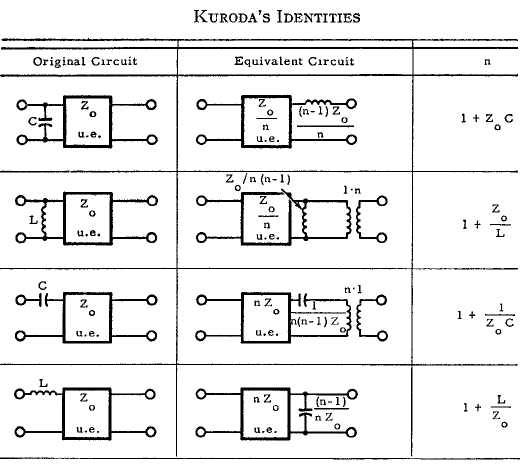
\includegraphics[width=\imagewidth]{images/kuroda-identities}
    \caption{Kuroda-Identit\"aten}
    \label{fig:kuroda-identities}
\end{figure}

In     der     Abbildung    \ref{fig:kuroda-identities}    sind    die     von
Kuroda\cite{ref:kuroda} formulierten Identit\"aten.  Damit  kann  zum Beispiel
mit   der   vierten  Identit\"at   eine   schlecht   realisierbare   erdfreie,
kurzgeschlossene  Stichleitung   in   eine   einfach  realisierbare  geerdete,
leerlaufende    Stichleitung    umgeformt    werden.    Wir   benützen   diese
Kuroda-Transformation,  um  den in  der  Richards-Transformation  entstandenen
Tiefpassfilter  in  eine  realisierbare  Topologie umzuformen.  Die  Abbildung
\ref{fig:kuroda-schieben}   zeigt   den   Vorgang   anhand   eines   einfachen
Tiefpass-Filters.

\begin{figure}[h!]
    \centering
    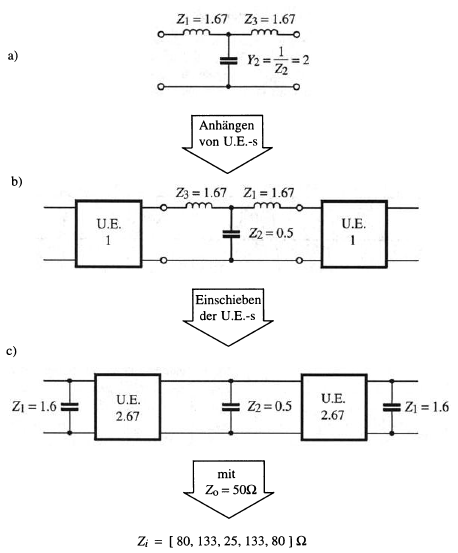
\includegraphics[width=.8\linewidth]{images/kuroda-schieben}
    \caption{Beispiel einer Umwandlung von schlecht realisierbaren Leitungsst\"ucken mithilfe der Kuroda-Transformation}
    \label{fig:kuroda-schieben}
\end{figure}

